%!TEX root=report.tex
\subsection{Kernel Principal Component Analysis (Kernel PCA)}

Before delving into kernel methods, the standard PCA method will briefly be recapped. PCA as introduced in this report was done via SVD ($X=U\Sigma V^T$); the columns of $U$ were the eigenvectors of $XX^T$ and the columns of $Z$ where $Z=U\Sigma$ constituted a basis in the PCA-vectorspace ($Z$); these columns were referred to as the principal components (PCs). 
Looking at the dependencies of $U$ it is apparent that the PCs will end up being linear combinations of basis in original input space $X$. 
In most cases this suffices but what if there are no linear relationships in the $X$ space, standard PCA won't be appropriate.
Below is a motivating example:

\begin{figure}[H]
\center
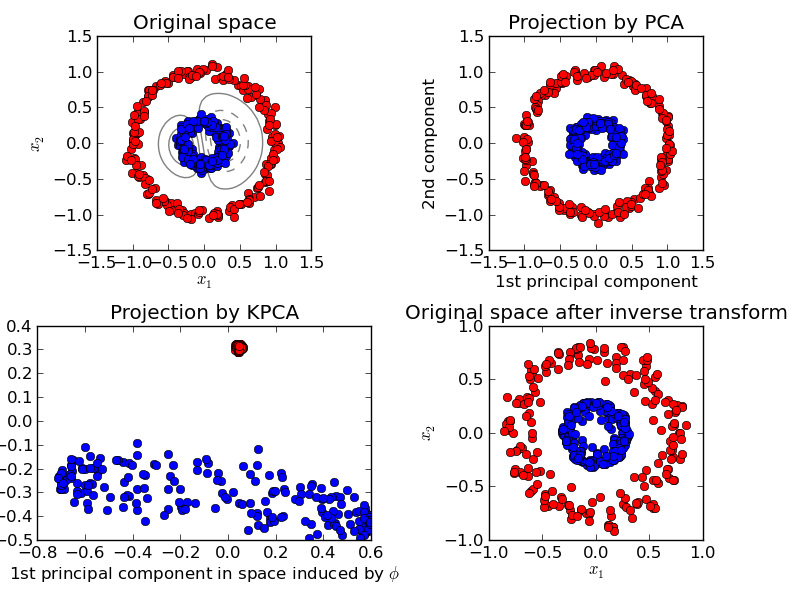
\includegraphics[width=\textwidth]{figures/kernel_pca_example.png}
	\caption{Motivating kernel PCA example. Image courtesy of scikit-learn (link in footnote)\footnote{http://scikit-learn.org/stable/auto_examples/decomposition/plot_kernel_pca.html}}
	\label{fig:motivation_kernelpca}
\end{figure}
